\documentclass[a4paper, 11pt]{article}


\usepackage{geometry}
 \geometry{
 a4paper,
 total={170mm,257mm},
 left=20mm,
 top=20mm,
 }
\usepackage{listings}
\usepackage{graphicx}
\graphicspath{ {./images/} }
\usepackage[utf8]{inputenc}
\usepackage[T1]{fontenc}
\usepackage[polish]{babel}
\usepackage{listings}
\usepackage{natbib}
\usepackage{indentfirst}
\usepackage{hyperref}
\hypersetup{
    colorlinks=true,
    linkcolor=blue,
    filecolor=magenta,      
    urlcolor=cyan,
}
\lstdefinelanguage{scala}{
  morekeywords={abstract,case,catch,class,def,%
    do,else,extends,false,final,finally,%
    for,if,implicit,import,match,mixin,%
    new,null,object,override,package,%
    private,protected,requires,return,sealed,%
    super,this,throw,trait,true,try,%
    type,val,var,while,with,yield},
  otherkeywords={=>,<-,<\%,<:,>:,\#,@},
  sensitive=true,
  morecomment=[l]{//},
  morecomment=[n]{/*}{*/},
  morestring=[b]",
  morestring=[b]',
  morestring=[b]"""
}
\title{%
  Gilded Rose \\
  \large Projekt sklepu z przedmiotami - refactoring na przykładzie języka Scala}
\author{Dawid Bińkuś, 246793}
\begin{document}
\maketitle
\section{Wstęp}
\subsection{Źródła}
Przykład refactoryzacji w języku Scala został wykonany na podstawie projektu GildedRose.
\begin{itemize}
	\item Oryginalna treść projektu: \href{https://github.com/emilybache/GildedRose-Refactoring-Kata}{https://github.com/emilybache/GildedRose-Refactoring-Kata}
	\item Rozwiązanie zadania zaimplementowane w języku Scala \\\href{https://github.com/inql/zjp-assignment}{https://github.com/inql/zjp-assignment}
\end{itemize}
\subsection{Narzędzia wykorzystane do dokonania refactoryzacji kodu}
W celu rozwiązania zadania zostały wykorzystane następujące narzędzia:
\begin{itemize}
 \item Scalatest, wykorzystywany do implementacji testów jednostkowych: \href{http://www.scalatest.org/}{http://www.scalatest.org/}
 \item Scoverage, dodatek wykorzystywany do określenia pokrycia kodu przez testy:\\ \href{https://github.com/scoverage/sbt-scoverage}{https://github.com/scoverage/sbt-scoverage}
 \item Scapegoat, dodatek służący do określenia jakości kodu: \href{https://github.com/sksamuel/scapegoat}{https://github.com/sksamuel/scapegoat}
 \item SonarQube, narzędzie używane do analizy projektu wraz z dodatkiem \textit{sbt-sonar} wykorzystywanym do integracji w/w narzędzia z projektem: \href{https://github.com/mwz/sbt-sonar}{https://github.com/mwz/sbt-sonar}
\end{itemize}
\subsection{Omówienie kodu początkowego}
\subsubsection{Struktura klas}
Początkowa implementacja GildedRose składa się z dwóch klas:
\begin{itemize}
 \item \textbf{Item} - Klasa określająca strukturę przedmiotów w systemie - posiadaja ona informacje o nazwie przedmiotu, jakości oraz terminie w którym dany przedmiot ma być sprzedany.
 \item \textbf{GildedRose} - Klasa przechowująca logikę systemu GildedRose - zawiera tablicę przedmiotów obecnych w systemie. Dodatkowo, zawiera metodę umożliwiającą zaktualizować stan wszystkich przedmiotów.
\end{itemize}
\subsubsection{Omówienie logiki systemu GildedRose}
Zamysł logiki zaimplementowanej do systemu prezentuje się w sposób następujący:
\begin{enumerate}
 \item Sprawdzenie typu przedmiotu bazując na jego nazwie.
 \item Zmienienie jakości przedmiotu bazując na jego typie.
 \item Obniżenie terminu sprzedaży na przedmiocie.
\end{enumerate}
W zależności od typu przedmiotu mogą wystąpić dodatkowe efekty podczas aktualizacji danych, np. dla przedmiotu typu \textit{Aged Brie} jakość rośnie im dłużej jest magazynowany (tj. wartość terminu sprzedaży jest mniejsza niż zero), a właściwości przedmiotu typu \textit{Legendary} są stałe niezależnie od czasu spędzonego w systemie.
\subsubsection{Omówienie początkowej jakości kodu}
Początkowa logika systemu została napisany w sposób bardzo prosty a zarazem skomplikowany do zrozumienia. Cała logika opiera się na iteracji po poszczególnych przedmiotach w systemie a następnie zastosowaniu zmian zdefiniowanych w dokumentacji. Realnym problemem okazuje się sposób w jaki wykonywana jest ta czynność. Cała logika opiera się na skomplikowanej strukturze wyrażeń warunkowych, które rozgałęziają się i zagnieżdżają ze sobą co znacznie zwiększa złożoność implementacji.\\
Po początkowym skanowanie za pomocą narzędzia SonarQube kwestia jakości kodu została wyjaśniona:
\begin{figure}[!tbh]
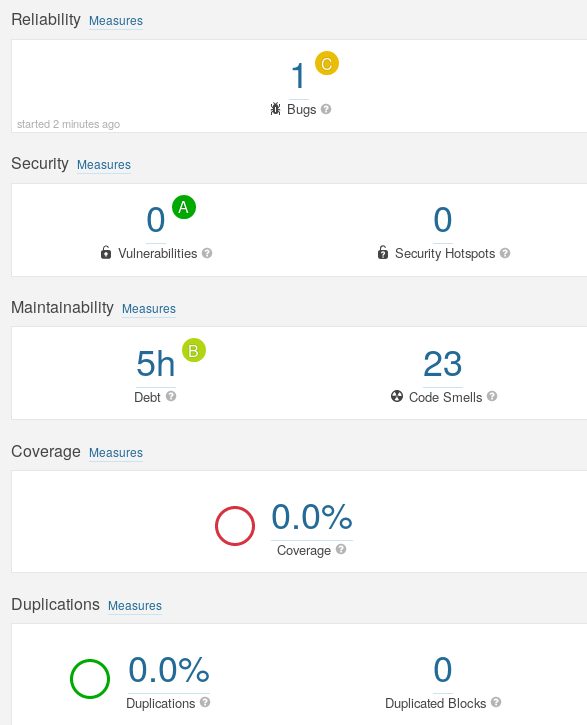
\includegraphics[width=8cm]{v01_ov}
\centering
\end{figure}\\
Bazując na rezultatach skanowania, znaczącym błędem mogącym prowadzić do nieprawidłowości było zerowanie wartości \textit{quality} produktu poprzez wykorzystanie danego wyrażenia:
\begin{lstlisting}[language=scala]
items(i).quality = items(i).quality - items(i).quality
\end{lstlisting}
Następnym obszarem wymagającym poprawy jest ogólnopojęta jakość kodu - SonarQube wykrył nieprawidłowości w postaci 23 \textit{Code Smells}. Dotyczyły one głównie braku odpowiedniego udokumentowania dla implementacji, zagnieżdżonych wyrażeń warunkowych oraz złożoności, utrudniającej zrozumienie instrukcji wykonywanych w programie.
\section{Omówienie procesu refactoryzacji}
W celu rozpoczęcia procesu refactoryzacji niezbędne było określenie jakie kolejne kroki należy podjąć by osiągnąć postawiony cel. Rozwój projektu podzieliłem na następujące etapy:
\begin{enumerate}
 \item Implementacja testów jednostkowych - zgodnie z zasadą \textbf{TDD}, chcemy mieć ciągłą kontrolę na poprawnością implementacji - w początkowej wersji projektu, testy nie były zaimplementowane.
 \item Uproszczenie głównej funkcji odpowiedzialnej za logikę projektu - by uczynić kod bardziej czytelnym i mniej skomplikowanym, należy całkowicie zmienić jego strukturę działania. Etap jest ten również przygotowaniem do kolejnej fazy.
 \item Implementacja nowej funkcjonalności - treść zadania wymaga dodania obsługi przedmiotów typu \textit{conjured} - po uproszczeniu logiki aplikacji zadanie to powinno być znacznie prostsze.
\end{enumerate}
\subsection{Implementacja testów}
Do implementacji testów wykorzystana została biblioteka \textit{Scalatest} - umożliwia ona pisanie testów w prosty sposób a wykonywane instrukcje powinny być zrozumiane również przez osobę nietechniczną. Dostarczona implementacja testów sprawdzała nieistotną w kontekście aplikacji funkcjonalność - możliwość zmiany przedmiotu po zaktualizowaniu wartości.
Początkowy kod prezentował się w sposób następujący:
\begin{lstlisting}[language=scala]
 class GildedRoseTest  extends FlatSpec with Matchers {
      it should "foo" in {
        var items = Array[Item](new Item("foo", 0, 0))
        val app = new GildedRose(items)
        app.updateQuality()
        (app.items(0).name) should equal ("fixme")
      }
}
\end{lstlisting}
W celu napisania nowej implementacji testów, pozbyto się całkowicie starej implementacji i zastosowano nową, wykorzystującą moduły \textit{FunSpec} oraz \textit{BeforeAndAfterEach}. Pierwszy z nich posłużył nam do ustruktoryzowania procedur testowych (testy napisane w ten sposób można podzielić według testowanego obszaru i konkretnego zachowania w myśl zasday \textbf{BDD}). Drugi zaś umożliwił zaimplementowanie metody \textit{beforeEach}, która przygotowywała stan systemu przed wykonaniem operacji określonych w teście.\\
Początkowa definicja testów prezentuje się w sposób następujący:
\begin{lstlisting}[language=scala]
class GildedRoseTest extends FunSpec with BeforeAndAfterEach {

  var regular, agedBrie, sulfuras, backstage: Item = _
  var gildedRose: GildedRose = _

  override def beforeEach(): Unit = {
    regular = new Item("regular", 7, 7)
    agedBrie = new Item("Aged Brie", 15, 15)
    sulfuras = new Item("Sulfuras, Hand of Ragnaros", 30,80)
    backstage = new Item("Backstage passes to a TAFKAL80ETC concert", 11, 9)

    gildedRose = new GildedRose(Array(regular,agedBrie,sulfuras,backstage))
  }
\end{lstlisting}
Po przygotowaniu systemu do wykonywania testów poprzez wstrzyknięcie mu niezbednych danych, należało przejść do implementacji zachowań do sprawdzenia.
Za pomocą instrukcji \textit{describe} określony został obszar testów (system GildedRose), następnie za pomocą instrukcji \textit{it} zdefiniowane zostały testy bazujące na określonych oczekiwanych zachowaniach systemu. Przykładowe testy prezentują się w sposób następujący:
\begin{lstlisting}[language=scala]
  describe("GildedRose"){

    it("should degrade item's quality by one when the day ends"){
      gildedRose.updateQuality()
      assertResult(6)(regular.quality)
    }

    it("should reduce item's sellIn by one then the day ends"){
      gildedRose.updateQuality()
      assertResult(6)(regular.sellIn)
    }

    it("should degrade item's quality twice when sellIn reached zero"){
      regular.sellIn = 0
      gildedRose.updateQuality()
      assertResult(5)(regular.quality)
    }

    it("should item's quality never reach zero"){
      regular.quality = 0
      gildedRose.updateQuality()
      assertResult(0)(regular.quality)
    }
\end{lstlisting}
Po przygotowaniu wszystkich testów, należało przystąpić do wykonania testowego uruchomienia. Wszystkie testy były uruchamiane zarówno lokalnie jak i z użyciem kontenera tworzonego na witrynie github.com - repozytorium projektu zostało skonfigurowane w taki sposób by każda aktualizacja wiązała się z wykonaniem całej sekwencji testowej.
\begin{figure}[!tbh]
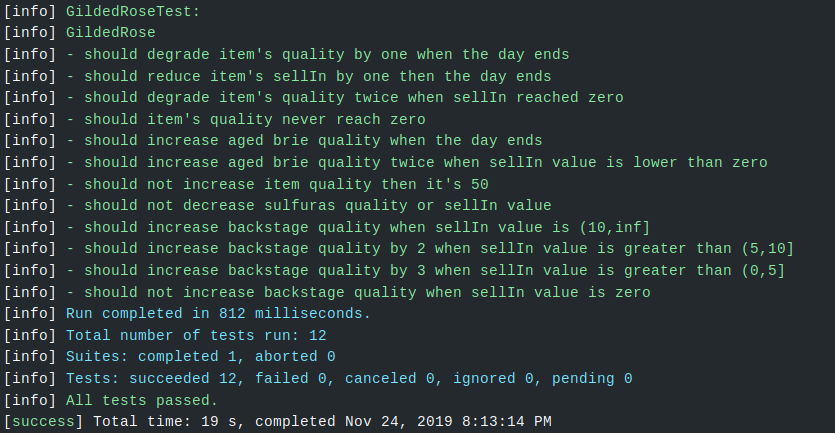
\includegraphics[width=8cm]{tests}
\centering
\end{figure}\\
Dzięki zaimplementowaniu testów jednostkowych, upewniliśmy się, że implementacja systemu mimo wątpliwej jakości, działa tak jak zakładaliśmy. Umożliwia to przejście do kolejnego etapu refactoryzacji.
Dodatkowo, osiągnięte zostało pokrycie kodu w postaci 100\% instrukcji zawartych w systemie GildedRose
\subsection{Upraszczanie kodu}
Implementacja systemu składająca się z szeregu zagnieżdżonych zapytań \textit{if} znacząco utrudniała zrozumienie kodu i znacznie ograniczała jego modularność oraz możliwość rozwinięcia jego zadań. 
By dokonać prawidłowego dokonania refactoryzacji kodu, należało dokładnie go przeanalizować a następnie podzielić go na mniejsze części by całość rozwiązania była bardziej spójna.
W przypadku projektu GildedRose, pierwszym krokiem było wydzielenie funkcji odpowiedzialnej za aktualizację jakości produktu, ponieważ to właśnie ta operacja była najbardziej narażona na nieprawidłowe zmiany. Treść nowo dodanej funkcji prezentowała się następująco:
\begin{lstlisting}[language=scala]
  def setMaxQuality(item: Item, updateValue: Int, maxQuality: Int): Item = {
    item.quality += updateValue
    item.quality = item.quality min maxQuality
    item
  }
\end{lstlisting}
Udało nam się już wydzielić część logiki z systemu GildedRose. Następnym krokiem było użycie go we właściwej już implementacji. Jest to również idealny moment by zmienić całą strukturę decydowania o aktualizacji stanu przedmiotu. Najrozsądniejszym rozwiązaniem okazało się reimpementacja klasy \textit{Item} na tzw. \textit{klasę przypadku} - specjalny rodzaj klasy, stworzony do kreowania takich obiektów jak np. przedmioty w bazie danych. Umożliwia on również zastosowanie tzw. zastosowania wzorca (ang. pattern matching) by stworzyć implementację nieopartą o zagnieżdżone zapytania if - co za tym idzie - ze znacznie zmniejszoną złożonością.
\begin{lstlisting}[language=scala]
case class Item(val name: String, var sellIn: Int, var quality: Int)
\end{lstlisting}
Po aktualizacji pliku GildedRose.scala, implementacja prezentuje się następująco:
\begin{lstlisting}[language=scala]
  def updateQuality(): Unit = {
    items.foreach {
      case Item("Sulfuras, Hand of Ragnaros", _, _) =>
      case item@Item("Aged Brie", sellIn, quality) if quality <= 50 & sellIn >= 0 =>
        item.sellIn -= 1
        setMaxQuality(item, 1, 50)
      case item@Item("Aged Brie", sellIn, quality) if quality <= 50 & sellIn < 0 =>
        item.sellIn -= 1
        setMaxQuality(item, 2, 50)
      case item@Item("Backstage passes to a TAFKAL80ETC concert", sellIn, quality) if quality < 50 && sellIn > 10 =>
        item.sellIn -= 1
        setMaxQuality(item, 1, 50)
      case item@Item("Backstage passes to a TAFKAL80ETC concert", sellIn, quality) if quality < 50 && sellIn > 5 =>
        item.sellIn -= 1
        setMaxQuality(item, 2, 50)
      case item@Item("Backstage passes to a TAFKAL80ETC concert", sellIn, quality) if quality < 50 && sellIn > 0 =>
        item.sellIn -= 1
        setMaxQuality(item, 3, 50)
      case item@Item("Backstage passes to a TAFKAL80ETC concert", sellIn, _) if sellIn <= 0 =>
        item.sellIn -= 1
        item.quality = 0
      case item@Item(_, sellIn, quality) if sellIn > 0 && quality > 0 =>
        item.sellIn -= 1
        item.quality -= 1
      case item@Item(_, sellIn, quality) if sellIn <= 0 && quality > 0 =>
        item.sellIn -= 1
        item.quality -= 2
      case _ =>
    }
  }
\end{lstlisting}
Dzięki zastosowaniu pattern matching, jakość i struktura kodu została znacznie usprawniona, jednocześnie pozostawiając implementację niezmienną. Ostatnim krokiem było wydzielenie zmiennych stałych dla nazw przedmiotu, by ułatwić przyszłą pracę z kodem źródłowym systemu.
\subsection{Implementacja nowej funkcjonalności}
Następnym etapem refactoryzacji kodu było dodanie nowej funkcjonalności zdefiniowanej w treści zadania. Zakładała ona dodanie nowego typu przedmiotu: \textit{conjured}, którego jakość spada każdego dnia o 2. W przypadku gdy termin sprzedaży minął, wartość ta spada dwukrotnie.
Pracę nad dodaniem implementacji rozpoczęto od zdefiniowania podstawowych testów jednostkowych - w myśl zasady \textbf{TDD} oraz \textbf{BDD}. 
\begin{lstlisting}[language=scala]
    it("should degrade conjured quality by two when the day ends"){
      gildedRose.updateQuality()
      assertResult(10)(conjured.quality)
    }

    it("should degrade conjured quality twice as normal if sellIn <=0"){
      conjured.sellIn = 0
      gildedRose.updateQuality()
      assertResult(8)(conjured.quality)
    } 
\end{lstlisting}
Dzięki refactoryzacji kodu, dodanie nowej funkcjonalności okazało się bardzo proste. Wystarczyło dodać kolejne instrukcje do głównej funkcji \textit{UpdateQuality}.
\begin{lstlisting}[language=scala]
...
case item@Item(Conjured, sellIn, quality) if quality > 0 && sellIn > 0 =>
    item.sellIn -= 1
    item.quality -=2
case item@Item(Conjured, sellIn, quality) if quality > 0 && sellIn <= 0 =>
    item.sellIn -= 1
    item.quality -= 4
...
\end{lstlisting}
Po dokonaniu implementacji, pozostało nam dodać kilka komentarzy w plikach źródłowych projektu by był on bardziej zrozumiały dla innych osób z nim pracujących, np.
\begin{lstlisting}[language=scala]
   /**
   * A function to avoid exceeding maximum quality of given item.
   * @param item Item to be checked
   * @param updateValue Value to be added to the item's quality.
   * @param maxQuality Maximum quality for given item.
   * @return
   */
  def setMaxQuality(item: Item, updateValue: Int, maxQuality: Int): Item = {
    item.quality += updateValue
    item.quality = item.quality min maxQuality
    item
  }

\end{lstlisting}

\subsection{Podsumowanie}
Teraz, gdy dodatkowa funkcjonalność została zaimplementowana, należy podsumować to co udało nam się osiągnąć podczas procesu refactoryzacji projektu GildedRose.
\begin{figure}[!tbh]
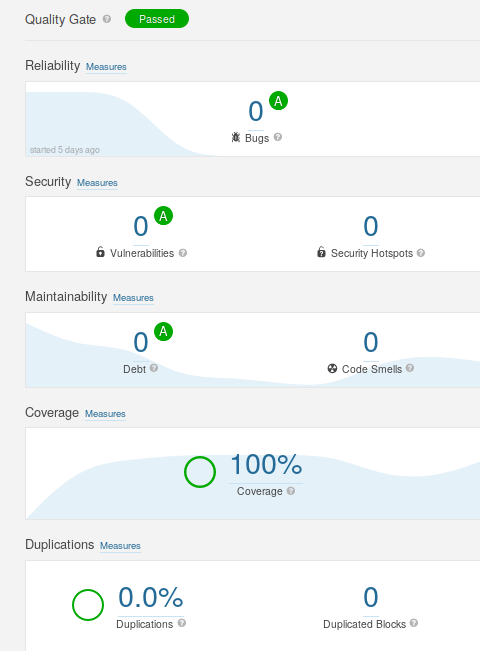
\includegraphics[width=4cm]{v1_ov}
\centering
\end{figure}\\
Jak można zauważyć wszystkie znaczące błędy oraz \textit{code smells} zostały naprawione. Dodatkowo pokrycie kodu przez testy jednostkowe pozostało niezmienione - znajduje się na poziomie 100\%.
\section{Dalsze usprawnienia}
Kod otrzymany w wyniku wykonanych zmian jest poprawny, aczkolwiek daleko mu do ideału. Brakuje mu skalowalności - każda nowa funkcjonalność wymaga zmiany głównej funkcji programu, co może powodować do błędów w przyszłości. Dodatkowo nie spełnia on warunków paradygmatów obiektowych oraz funkcjonalnych - Scala jest językiem który potrafi pogodzić te dwa paradygmaty, dlatego też w tym rozdziale zajmiemy się dalszymi usprawnieniami projektu GildedRose. Składają się one na:
\begin{enumerate}
 \item Wydzielenie logiki kodu za pomocą ekstrakcję zachowań poszczególnych przedmiotów.
 \item Umożliwienie sprawne tworzenie nowych zachowań z zachowaniem domyślnych właściwości nowo utworzonych przedmiotów.
 \item Reimplementacja głównej logiki by stała się niezależna i odporna na potencjalne zmiany.
\end{enumerate}
\subsection{Wydzielenie logiki kodu}
Podczas refactoryzacji kodu zauważalne stały się zależności między zachowaniami poszczególnych przedmiotów. Podczas operacji aktualizacji danych nadpisywane są dwa z trzech pól - termin sprzedaży oraz jakość obiektu. Dodatkowo większość z nich współdzieli implementację niektórych zachowań.\\
Te obserwacje umożliwiły podzielenie zachowań według następującego wzorca:
\begin{enumerate}
 \item Zachowanie bazowe, które definiuje sposób aktualizacji pól obiektów.
 \item Zachowania dziedziczące po bazowym, które mogą być całkowicie zależne od bazowego, zachowywać się w sposób niezależny bądź cześciowo implementować zachowanie bazowe.
\end{enumerate}
W późniejszych podrozdziałach podjęty zostanie temat dalszej pracy nad systemem GildedRose
\subsubsection{Potencjał dziedziczenia zachowań przedmiotów}
Zachowanie bazowe zostało zaimplementowane za pomocą tzw. \textit{klasy abstrakcyjnej} w której zdefiniowane zostały operacje współdzielone przez poszczególne przedmioty.
\begin{lstlisting}[language=scala]
 /**
 * Abstract class which create behaviour based on the item name.
 * @param item Item to create a behaviour for.
 */
abstract class Behaviour(item: Item) {

  val maxQuality = 50
  val minQuality = 0

  def update(): Unit = {
    updateQualityValue()
    updateSellInValue()

    item.quality = if (item.quality > maxQuality)  maxQuality
      else if (item.quality < minQuality) minQuality
        else item.quality
  }


  protected def updateQualityValue(): Unit

  protected def updateSellInValue(): Unit = item.sellIn -= 1

}
\end{lstlisting}
Następnie, utworzone zostały klasy poszczególnych przedmiotów, które dziedziczyły po klasie abstrakcyjnej \textit{Behaviour}. W zależności od potrzeb, dane podklasy nadpisywały zachowania swojego rodzica bądź czerpały implementację bezpośrednio od niego.
\begin{lstlisting}[language=scala]
 class DefaultBehaviour(item: Item) extends Behaviour(item){
  override protected def updateQualityValue(): Unit = {
    item.quality = if (item.sellIn <= 0) item.quality - 2 else item.quality - 1
  }
}

class BackstageBehaviour(item: Item) extends Behaviour(item){
  override protected def updateQualityValue(): Unit = {
    item.quality = if (item.sellIn < 6) item.quality + 3
      else if (item.sellIn < 11) item.quality + 2
        else item.quality + 1
  }

  override protected def updateSellInValue(): Unit = {
    super.updateSellInValue()
    item.quality = if (item.sellIn < 0) 0 else item.quality
  }
}
\end{lstlisting}
Warto nadmienić tutaj fakt, że same klasy zachowań zostały napisane w taki sposób by był swoistym opakowaniem dla poszczególnych przedmiotów. Same w sobie nie zwracają żadnych wartości, jedyne co wykonują to pobieranie przedmiotu w konstruktorze oraz dokonywanie na nim niezbędnych operacji. Dodatkowo, wykorzystana została tutaj jedna z cech języka programowania Scala - wyrażenia traktowane w językach obiektowych jako imperatywne (takie jak np. \textbf{for, if}, tutaj są funkcjami i zwracają wartość. Dzięki tej właściwości wyrażenie
\begin{lstlisting}[language=scala]
item.quality = if (item.sellIn < 0) 0 else item.quality
\end{lstlisting}
jest akceptowane przez maszynę wirtualną Javy - w efekcie przypisuje do pola żądaną wartość w zależności od danego warunku.
\subsubsection{Wzorzec projektowy fabryka}
Kiedy poszczególne zachowania zostały już zdefiniowane pozostaje kolejny problem do rozwiązania - przypisywanie przedmiotów do poszczególnych wzorców. W tym celu utworzony został obiekt \textit{ItemFactory} wraz ze zdefiniowaną funkcją \textit{update}. Jej zadaniem jest zdefiniowanie zachowania na podstawie jego nazwy. Implementacja prezentuje się w sposób następujący:
\begin{lstlisting}[language=scala]
 object ItemFactory {
  def create(item: Item): Behaviour = item.name match {
    case "Sulfuras, Hand of Ragnaros" => new LegendaryItemBehaviour(item)
    case "Aged Brie" => new AgedBrieBehaviour(item)
    case "Backstage passes to a TAFKAL80ETC concert" => new BackstageBehaviour(item)
    case "conjured" => new ConjuredBehaviour(item)
    case _ => new DefaultBehaviour(item)
  }
}
\end{lstlisting}
Do rozpatrzenia odpowiedniego zachowania dla danego przedmiotu zastosowane zostało dopasowanie wzorca.
\subsubsection{Finalizacja}
W celu wykorzystania nowo utworzonej implementacji zachowań, należało zmienić główną funkcję obsługującą logikę GildedRose. Dotychczasowa iteracja oraz dopasowanie wzorca nie jest już potrzebne, dlatego cała obsługa przedmiotów w systemie została skrócona do czysto funkcyjnej postaci:
\begin{lstlisting}[language=scala]
 class GildedRose(val items: Array[Item]) {
  /**
   * A function which maps all given items into Behaviour wrapper and updates its values.
   */
  def updateQuality(): Unit = {
    items.map(ItemFactory.create).foreach(_.update())
  }
}
\end{lstlisting}
\section{Podsumowanie}
Finalna analiza projektu za pomocą narzędzia SonarQube prezentuje się w sposób następujący:
\begin{figure}[!tbh]
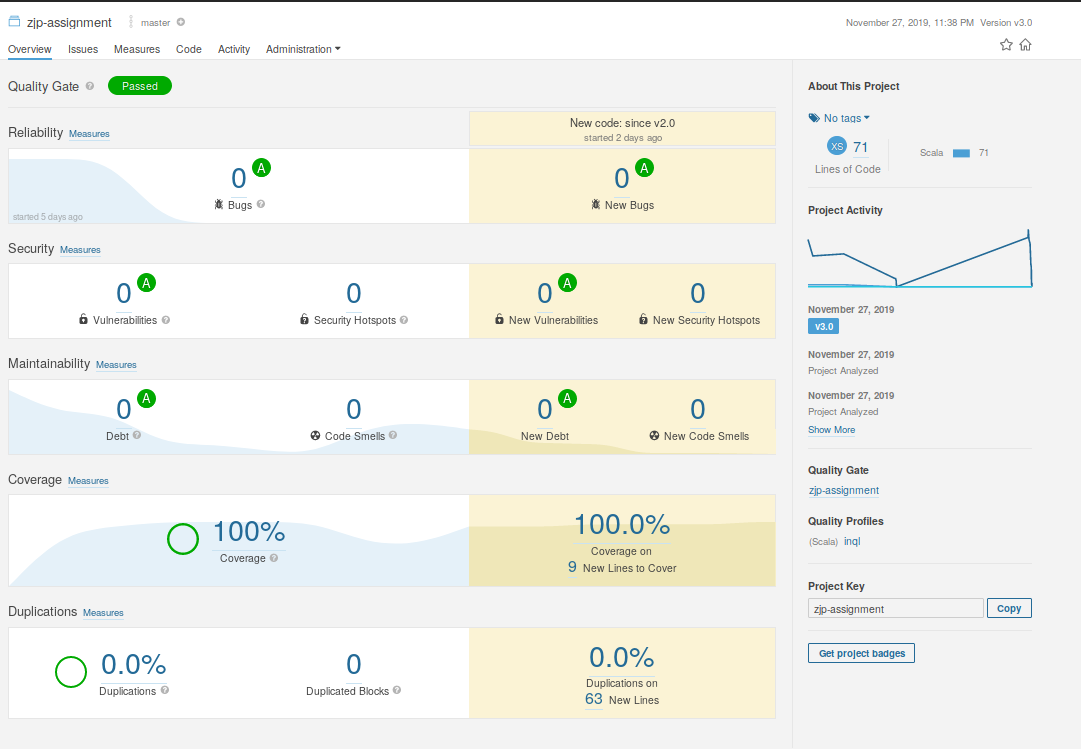
\includegraphics[width=16cm]{final_ov}
\centering
\end{figure}\\
Jak widać na załączonym raporcie, wszystkie początkowe problemy związane zarówno z poprawnością implementacji jak i jej jakością zostały naprawione. Testy zgodnie z założeniem pokrywają 100\% przypadków oraz w kodzie nie znajdują się żadne duplikaty. DOdatkowo udało się implementację znacznie uprościć i skrócić, dzięki zastosowaniu podeścia modularnego w postaci obiektów reprezentujacych zachowanie jak i uzyciu paradygmantów funkcyjnych.
Przystąpmy teraz do analizy rozwoju projektu na przestrzeni poszczególnych wydań.
\begin{figure}[!tbh]
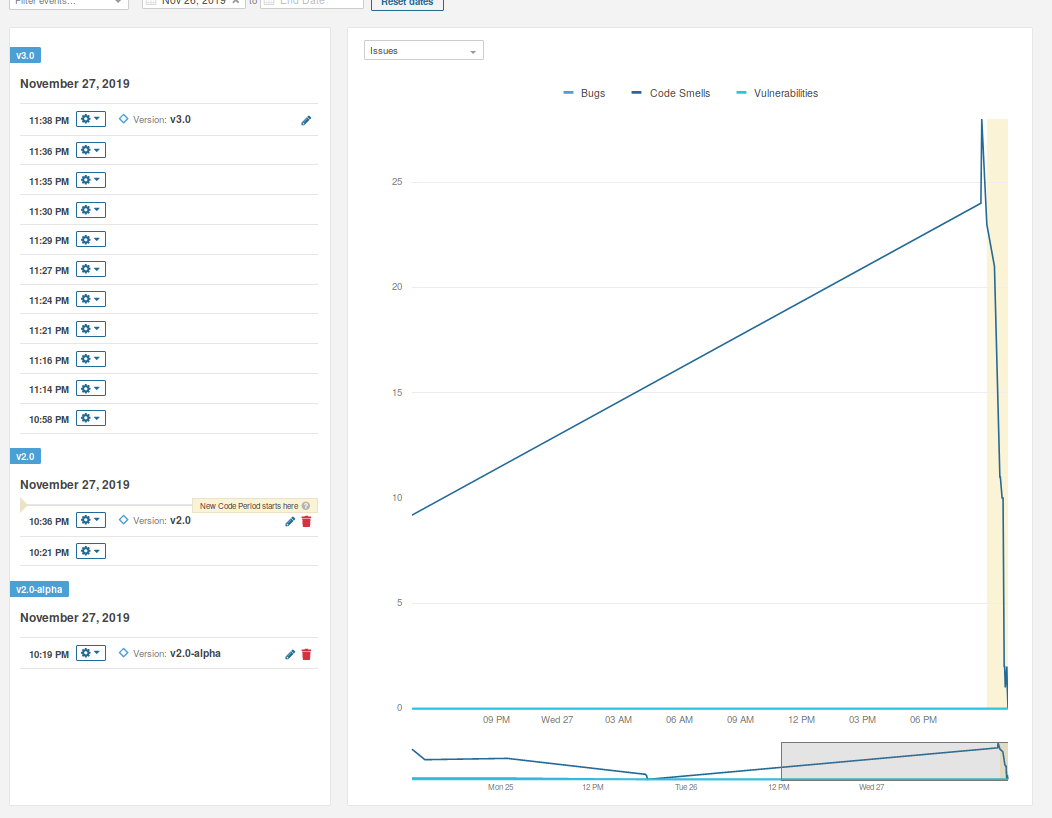
\includegraphics[width=16cm]{final_issues}
\centering
\end{figure}\\
Na załączonych wykresach widać spadek problemów z kodem źródłowym projektem na przestrzeni posczególnych wersji. Duża część z nich była generowana w trakcie procesu refactoryzacji, lecz równie sprawne były one eliminowane.
\begin{figure}[!tbh]
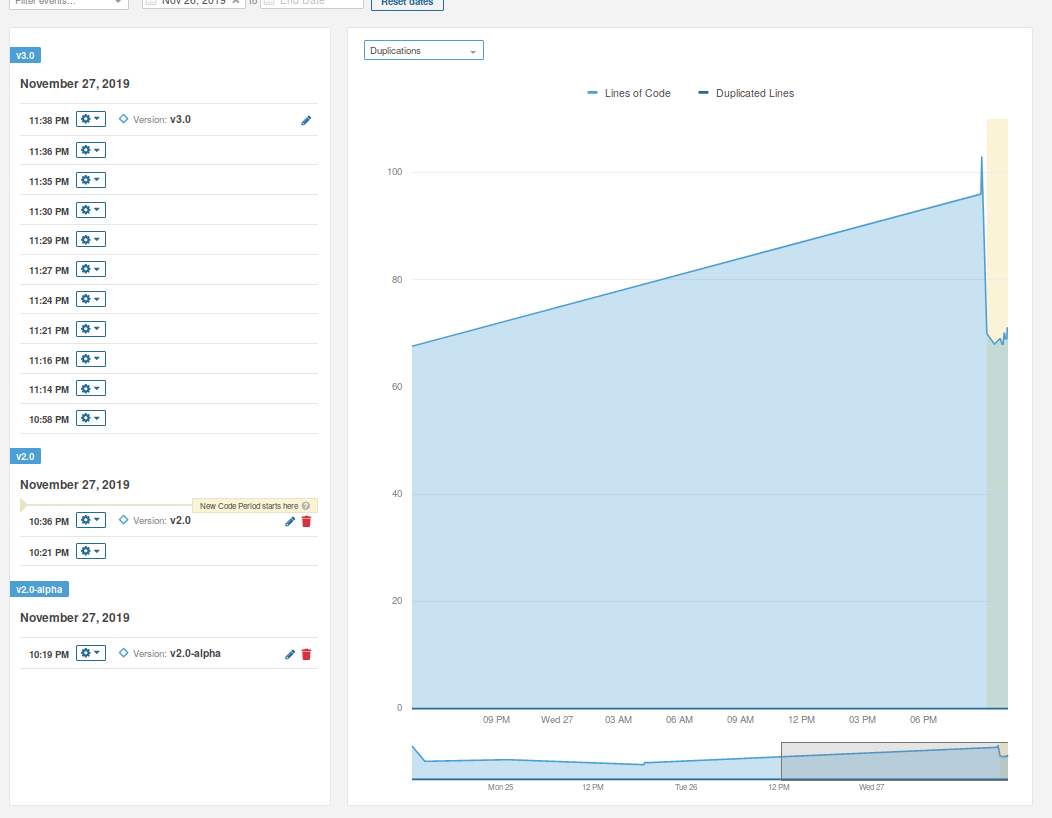
\includegraphics[width=16cm]{final_dup}
\centering
\end{figure}\\
Zmniejszyła się również ilość linii co udowadnia dużą złożoność kodu wyjściowego oraz poprawność zastosowanego rozwiązania.
\end{document}
